\section{Program iOvčar IZIDOR}

Za učenje in testiranje modelov smo pripravili program, ki smo ga poimenovali \textit{iOvčar IZIDOR}. Program je napisan v programskem jeziku $C\#$, za vizualizacijo smo uporabljali program Unity in za spodbujevano učenje paket ML Agents\footnote{Pri učenju nam je bila v veliko pomoč spletna stran \url{https://www.immersivelimit.com} [ogled 9.\ 3.\ 2021].}. Program nam je omogočal grafični prikaz simulacije in beleženje rezultatov. Na slikah~\ref{fig:pasnik} in~\ref{fig:meni} si lahko ogledamo izgled simulacijskega okolja.

V programu so modeli vodenja psa ovčarja običajno poimenovani na drugačen način. Ročno razviti model je imenovan "Voronoi", model razvit z genetskim algoritmom je "AI1" in model z adaptivnim genom je "AI2".

\begin{figure}[ht]  % ali t za na vrhu ali h! za točno tukaj
	\centering
	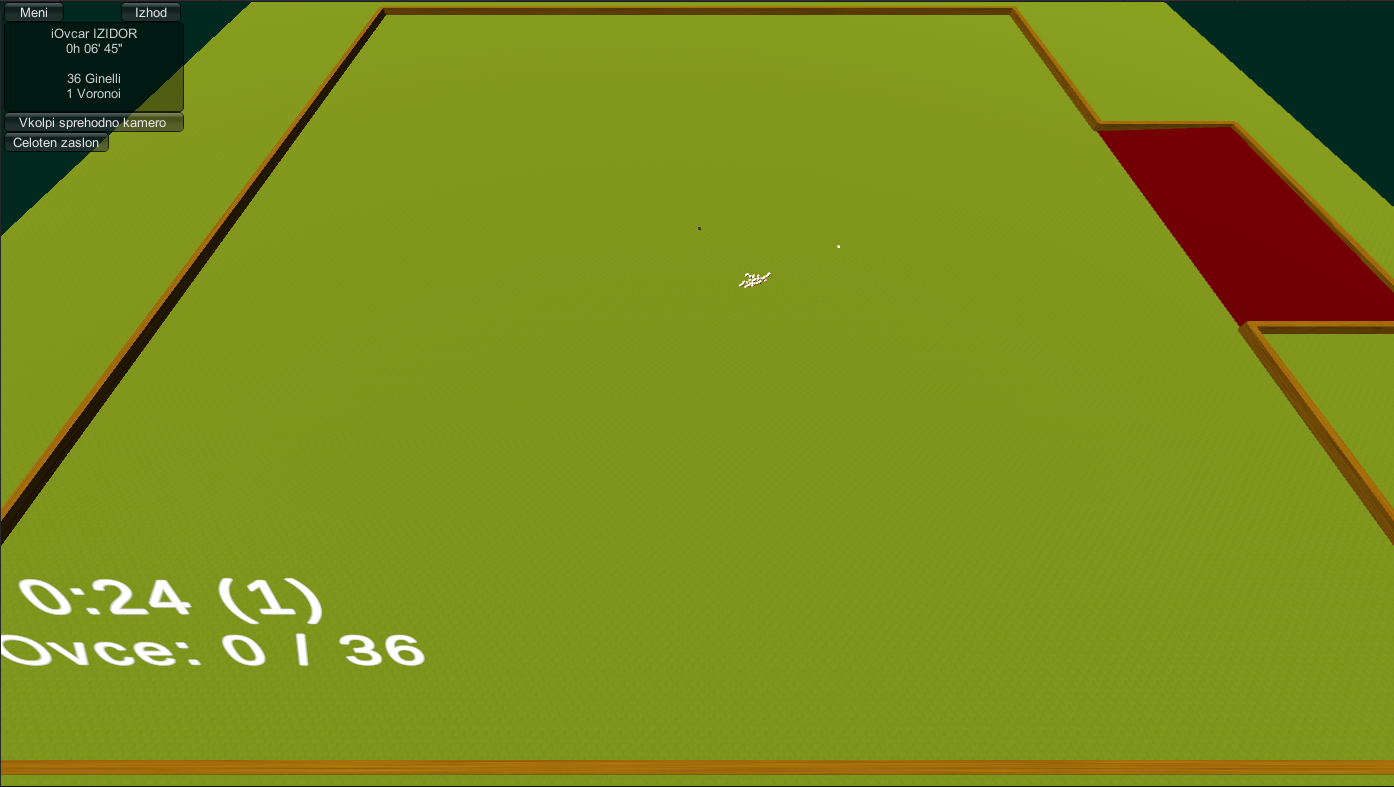
\includegraphics[width=0.7\textwidth]{../poglavja/images/obicajen-pogled.png}
	\caption[Pogledi med simulacijo]{Običajen pogled med simulacijo. Program nam omogoča tudi pogled od zgoraj in izza izbranega ovčarja.} % narejena je s programom Inkscape
	\label{fig:pasnik}
\end{figure}

\begin{figure}[ht]  % ali t za na vrhu ali h! za točno tukaj
	\centering
	
\includegraphics[width=0.8\textwidth]{../poglavja/images/meni.png}
	\caption[Meni programa]{Meni za izbiro nastavitev v programu.} % narejena je s programom Inkscape
	\label{fig:meni}
\end{figure}
